\documentclass[12pt]{article}

\usepackage{sbc-template} 
\usepackage{graphicx,url}
\usepackage{url}
\usepackage[brazil]{babel} 
\usepackage[utf8]{inputenc} 
\usepackage[T1]{fontenc}
\usepackage[normalem]{ulem}
\usepackage[hidelinks]{hyperref}
\usepackage[square,authoryear]{natbib}
\usepackage{amssymb} 
\usepackage{mathalfa} 
\usepackage{algorithm} 
\usepackage{algpseudocode} 
\usepackage[table]{xcolor}
\usepackage{array}
\usepackage{titlesec}
\usepackage{mdframed}
\usepackage{amsmath} 
\usepackage{booktabs}
\usepackage{listings}
\usepackage{xcolor}

\definecolor{codegreen}{rgb}{0,0.6,0}
\definecolor{codegray}{rgb}{0.5,0.5,0.5}
\definecolor{codepurple}{rgb}{0.58,0,0.82}
\definecolor{backcolour}{rgb}{0.95,0.95,0.92}
\lstdefinestyle{mystyle}{
    commentstyle=\color{codegreen},
    keywordstyle=\color{magenta},
    numberstyle=\tiny\color{codegray},
    stringstyle=\color{codepurple},
    basicstyle=\ttfamily\footnotesize,
    breakatwhitespace=false,
    breaklines=true,                 
    captionpos=b,                    
    keepspaces=true,                 
    numbers=left,                    
    numbersep=10pt,                  
    showspaces=false,                
    showstringspaces=false,
    showtabs=false,                  
    tabsize=2
}
\lstset{style=mystyle}

\urlstyle{same}

\newcolumntype{L}[1]{>{\raggedright\let\newline\\\arraybackslash\hspace{0pt}}m{#1}}
\newcolumntype{C}[1]{>{\centering\let\newline\\\arraybackslash\hspace{0pt}}m{#1}}
\newcolumntype{R}[1]{>{\raggedleft\let\newline\\\arraybackslash\hspace{0pt}}m{#1}}
\newcommand\Tstrut{\rule{0pt}{2.6ex}} 
\newcommand\Bstrut{\rule[-0.9ex]{0pt}{0pt}} 
\newcommand{\scell}[2][c]{\begin{tabular}[#1]{@{}c@{}}#2\end{tabular}}
\usepackage[nolist,nohyperlinks]{acronym}

\title{Trabalho 1 de Aprendizado de Máquina}

\author{Gabriel Ramos, Guilherme Vieira, Lucca Demichei\inst{1}}

\address{Pontifícia Universidade Católica do Rio Grande Do Sul - PUCRS
	\email{\{guilherme.camara, lucca.demichei, gabriel.ramos03\}@edu.pucrs.br}
}
\begin{document} 
	\maketitle
 
\section{Introdução}

\label{sec:introducao}
 
O aprendizado de máquina envolve a construção de modelos preditivos a partir de dados, e a diversidade de algoritmos disponíveis permite abordar uma vasta gama de problemas de classificação e regressão. Este trabalho tem como objetivo comparar três algoritmos de aprendizado supervisionado discutidos em aula — sendo eles a Árvore de Decisão, o K-Nearest Neighbors (KNN) e o Naive Bayes — com um quarto algoritmo gerado pelo modelo GPT-4 da OpenAI, desenvolvido sem o uso de bibliotecas como Scikit-learn. Ao longo da implementação, exploramos os fundamentos teóricos de cada técnica, discutindo seus prós e contras e analisando como esses algoritmos se comportam na prática. A comparação entre as implementações se concentra na eficiência, precisão, simplicidade e aplicabilidade dos algoritmos, buscando estabelecer paralelos com o conteúdo teórico discutido ao longo do curso.



\section{Implementação dos algoritmos pelo ChatGPT}
\label{sec:implementacao}

\subsection{K-NN}
\subsubsection{Prompt utilizado}
"Implemente um algoritmo do Knn em python sem usar scikit-learn"

\subsection{Resposta completa gerada pelo ChatGPT}

Aqui está uma implementação básica do algoritmo K-Nearest Neighbors (KNN) em Python, sem o uso da biblioteca 'scikit-learn'. Esse código implementa o KNN de forma simples e eficiente, usando apenas bibliotecas padrão do Python como 'math' e 'collections' para calcular as distâncias e determinar os vizinhos mais próximos.

Passos principais do KNN:
1. Calcular a distância entre o ponto de teste e todos os pontos de treino.
2. Selecionar os `k` vizinhos mais próximos com base nas distâncias.
3. Realizar a votação majoritária (para classificação) ou calcular a média (para regressão) entre os vizinhos selecionados.

Aqui está o código de exemplo:

\begin{verbatim}
import math
from collections import Counter

# Função para calcular a distância Euclidiana entre dois pontos
def euclidean_distance(point1, point2):
    return math.sqrt(sum((x - y) ** 2 for x, y in zip(point1, point2)))

# Implementação do algoritmo KNN
class KNN:
    def __init__(self, k=3):
        self.k = k
        self.data = None
        self.labels = None

    # Função para treinar o modelo com os dados de treino
    def fit(self, X_train, y_train):
        self.data = X_train
        self.labels = y_train

    # Função para prever o rótulo (classificação)
    def predict(self, X_test):
        predictions = []
        for test_point in X_test:
            # Calcular a distância de todos os pontos de treino
            distances = [(euclidean_distance(test_point, train_point), label)
                         for train_point, label in zip(self.data, self.labels)]
            # Ordenar as distâncias e pegar os k vizinhos mais próximos
            sorted_distances = sorted(distances)[:self.k]
            # Coletar os rótulos dos vizinhos mais próximos
            k_nearest_labels = [label for _, label in sorted_distances]
            # Votação majoritária
            most_common_label = Counter(k_nearest_labels).most_common(1)[0][0]
            predictions.append(most_common_label)
        return predictions

# Exemplo de uso
if __name__ == "__main__":
    # Dados de treino (4 amostras de 2 features)
    X_train = [[1, 2], [2, 3], [3, 4], [5, 6]]
    y_train = [0, 0, 1, 1]  # Rótulos correspondentes

    # Dados de teste (1 amostra de 2 features)
    X_test = [[1.5, 2.5]]

    # Instancia o modelo KNN
    knn = KNN(k=3)
    
    # Treina o modelo
    knn.fit(X_train, y_train)
    
    # Faz a previsão
    prediction = knn.predict(X_test)
    
    print("Predição:", prediction)
    
\end{verbatim}

Explicação:
- **euclidean\_distance**: Calcula a distância euclidiana entre dois pontos.
- **KNN**:
  - '\_\_init\_\_(self, k=3)': Inicializa o modelo com o número de vizinhos `k`.
  - 'fit(self, X\_train, y\_train)': Armazena os dados de treino e seus rótulos.
  - 'predict(self, X\_test)': Faz a previsão para novos dados de teste, calculando a distância de cada ponto de teste para todos os pontos de treino, selecionando os `k` mais próximos e retornando o rótulo mais comum (votação majoritária).
 Você pode alterar a função de distância para outras métricas, como distância de Manhattan, ou ajustar o valor de `k` conforme necessário.
 Se precisar de mais informações ou ajustes, estou à disposição!

\subsubsection{Algoritmo}
\lstinputlisting[language=python]{codigos/knn.py}

\subsection{Naive Bayes}
\subsubsection{Prompt utilizado}
"Implemente um algoritmo de Naive Bayes em python sem usar scikit-learn, ou seja, from scratch"

\subsection{Resposta completa gerada pelo ChatGPT}

Aqui está uma implementação básica de um classificador Naive Bayes "from scratch" em Python, sem usar `scikit-learn`. Essa abordagem é baseada no teorema de Bayes e na suposição de que as características são independentes entre si (daí o nome "Naive").

### Passos principais:
1. **Treinamento**: Calcular a probabilidade condicional de cada classe com base nas características (estimativas de máxima verossimilhança).
2. **Predição**: Para cada novo exemplo, calcular a probabilidade posterior de cada classe, dada a entrada, e selecionar a classe com a maior probabilidade.

Para simplificar, vamos implementar a versão para classificação binária ou multiclasse, assumindo que os atributos são contínuos (usaremos a função densidade de probabilidade Gaussiana).

### Implementação:

\begin{verbatim}
import numpy as np

class NaiveBayes:
    def fit(self, X_train, y_train):
        # Separar por classe
        self.classes = np.unique(y_train)
        self.mean = {}
        self.var = {}
        self.priors = {}
        
        # Para cada classe
        for c in self.classes:
            X_c = X_train[y_train == c]
            self.mean[c] = np.mean(X_c, axis=0)
            self.var[c] = np.var(X_c, axis=0)
            self.priors[c] = X_c.shape[0] / X_train.shape[0]

    # Função para calcular a densidade de probabilidade Gaussiana
    def gaussian_pdf(self, class_idx, x):
        mean = self.mean[class_idx]
        var = self.var[class_idx]
        numerator = np.exp(-(x - mean) ** 2 / (2 * var))
        denominator = np.sqrt(2 * np.pi * var)
        return numerator / denominator
    
    # Função para calcular a probabilidade posterior
    def predict(self, X_test):
        y_pred = [self._predict(x) for x in X_test]
        return np.array(y_pred)
    
    # Função interna que calcula a probabilidade posterior para um exemplo
    def _predict(self, x):
        posteriors = []
        
        for c in self.classes:
            prior = np.log(self.priors[c])  # Probabilidade a priori
            conditional = np.sum(np.log(self.gaussian_pdf(c, x)))  # Verossimilhança
            posterior = prior + conditional  # Posterior
            posteriors.append(posterior)
        
        return self.classes[np.argmax(posteriors)]  # Retorna a classe com maior probabilidade

# Exemplo de uso
if __name__ == "__main__":
    # Exemplo de dados: 2 features
    X_train = np.array([[1, 2], [2, 3], [3, 4], [4, 5], [5, 6]])
    y_train = np.array([0, 0, 1, 1, 1])

    X_test = np.array([[1.5, 2.5], [3.5, 4.5]])

    # Instancia o classificador Naive Bayes
    nb = NaiveBayes()
    
    # Treina o modelo
    nb.fit(X_train, y_train)
    
    # Faz a predição
    predictions = nb.predict(X_test)
    
    print("Predições:", predictions)
\end{verbatim}

Explicação:
1. **'fit(self, X\_train, y\_train)'**:
   - Calcula a média, a variância e as probabilidades a priori para cada classe. A suposição é que as características seguem uma distribuição normal (Gaussiana), então armazenamos a média e a variância de cada característica para cada classe.
   
2. **'gaussian\_pdf(self, class\_idx, x)'**:
   - Função que calcula a densidade de probabilidade Gaussiana, dada uma amostra, para uma determinada classe. Isso é utilizado para calcular a verossimilhança de uma amostra pertencer a uma classe.

3. **'predict(self, X\_test)'**:
   - Calcula a probabilidade posterior para cada classe e retorna a classe com a maior probabilidade.

4. **\_Exemplo de uso\_**:
   - No final, temos um exemplo de como o algoritmo pode ser utilizado, com um conjunto de treino simples e um conjunto de teste para fazer a predição.

Fórmulas:
- A densidade de probabilidade Gaussiana para cada atributo \( x\_i \) é calculada como:

  $P(x_i|c) = \frac{1}{\sqrt{2\pi \sigma_c^2}} \exp\left(-\frac{(x_i - \mu_c)^2}{2\sigma_c^2}\right)$
  
  Onde \( \mu_c \) e \( \sigma_c \) são a média e a variância da classe \( c \) para a característica \( x_i \).
  
- A probabilidade posterior é:

  $ P(c|x) \propto P(c) \prod_{i=1}^{n} P(x_i|c) $
  
 Se precisar de ajustes ou mais explicações, me avise!

\subsubsection{Algoritmo}
\lstinputlisting[language=python]{codigos/naivebayes.py}

\subsection{Árvore de Decisão}
\subsubsection{Prompt utilizado}
"Implemente um algoritmo de arvore de decisao em python sem usar scikit-leanr, ou seja, from scratch"

\subsection{Resposta completa gerada pelo ChatGPT}

Aqui está uma implementação de uma árvore de decisão do zero em Python, sem o uso da biblioteca 'scikit-learn'. A implementação utiliza o critério de **Gini** para dividir os dados:

Passo 1: Cálculo do Índice Gini
O índice Gini mede a impureza de uma divisão, ou seja, quão mista estão as classes.

Passo 2: Funções de Divisão
Precisamos de uma função para dividir os dados com base em um valor em uma coluna específica.

Passo 3: Construção da Árvore
A árvore de decisão é construída de forma recursiva, dividindo os dados até encontrar folhas puras ou atingir um critério de parada (como profundidade máxima).

Passo 4: Função de Previsão
Depois que a árvore é construída, a função de previsão é utilizada para classificar novas amostras.

Código:

\begin{verbatim}
import numpy as np

# Função para calcular o índice Gini de um grupo de amostras
def gini(groups, classes):
    # Número total de amostras
    n_instances = float(sum([len(group) for group in groups]))
    
    gini_index = 0.0
    for group in groups:
        size = len(group)
        if size == 0:
            continue
        score = 0.0
        # Proporção de cada classe no grupo
        for class_val in classes:
            p = [row[-1] for row in group].count(class_val) / size
            score += p * p
        gini_index += (1.0 - score) * (size / n_instances)
    
    return gini_index

# Função para dividir os dados em dois grupos com base em um valor específico de uma coluna
def test_split(index, value, dataset):
    left, right = [], []
    for row in dataset:
        if row[index] < value:
            left.append(row)
        else:
            right.append(row)
    return left, right

# Selecionar a melhor divisão do dataset
def get_split(dataset):
    class_values = list(set(row[-1] for row in dataset))
    b_index, b_value, b_score, b_groups = 999, 999, 999, None
    for index in range(len(dataset[0])-1):
        for row in dataset:
            groups = test_split(index, row[index], dataset)
            gini_index = gini(groups, class_values)
            if gini_index < b_score:
                b_index, b_value, b_score, b_groups = index, row[index], gini_index, groups
    return {'index': b_index, 'value': b_value, 'groups': b_groups}

# Criar um nó folha
def to_terminal(group):
    outcomes = [row[-1] for row in group]
    return max(set(outcomes), key=outcomes.count)

# Dividir os nós, criando sub-árvores de forma recursiva ou folhas
def split(node, max_depth, min_size, depth):
    left, right = node['groups']
    del(node['groups'])
    # Verificar se não há divisão
    if not left or not right:
        node['left'] = node['right'] = to_terminal(left + right)
        return
    # Verificar profundidade máxima
    if depth >= max_depth:
        node['left'], node['right'] = to_terminal(left), to_terminal(right)
        return
    # Processar o nó esquerdo
    if len(left) <= min_size:
        node['left'] = to_terminal(left)
    else:
        node['left'] = get_split(left)
        split(node['left'], max_depth, min_size, depth+1)
    # Processar o nó direito
    if len(right) <= min_size:
        node['right'] = to_terminal(right)
    else:
        node['right'] = get_split(right)
        split(node['right'], max_depth, min_size, depth+1)

# Construir uma árvore de decisão
def build_tree(train, max_depth, min_size):
    root = get_split(train)
    split(root, max_depth, min_size, 1)
    return root

# Fazer uma previsão com a árvore de decisão
def predict(node, row):
    if row[node['index']] < node['value']:
        if isinstance(node['left'], dict):
            return predict(node['left'], row)
        else:
            return node['left']
    else:
        if isinstance(node['right'], dict):
            return predict(node['right'], row)
        else:
            return node['right']

# Exemplo de uso
if __name__ == '__main__':
    # Dataset de exemplo: [característica1, característica2, ..., classe]
    dataset = [[2.771244718, 1.784783929, 0],
               [1.728571309, 1.169761413, 0],
               [3.678319846, 2.81281357, 0],
               [3.961043357, 2.61995032, 0],
               [2.999208922, 2.209014212, 0],
               [7.497545867, 3.162953546, 1],
               [9.00220326, 3.339047188, 1],
               [7.444542326, 0.476683375, 1],
               [10.12493903, 3.234550982, 1],
               [6.642287351, 3.319983761, 1]]

    # Definindo os parâmetros da árvore
    max_depth = 3
    min_size = 1

    # Construir a árvore
    tree = build_tree(dataset, max_depth, min_size)

    # Fazer previsões
    for row in dataset:
        prediction = predict(tree, row)
        print('Esperado=%d, Previsto=%d' % (row[-1], prediction))
\end{verbatim}

Explicação:
1. **gini**: Calcula o índice Gini para um conjunto de grupos.
2. **test\_split**: Divide o conjunto de dados em dois grupos com base no valor de uma característica.
3. **get\_split**: Encontra a melhor divisão possível do dataset, retornando o índice da coluna e o valor que proporcionam a menor impureza Gini.
4. **split**: Realiza a divisão recursiva dos nós.
5. **build\_tree**: Constrói a árvore de decisão.
6. **predict**: Faz previsões com base na árvore gerada.

Testando
O código usa um pequeno dataset para testar a construção da árvore e as previsões feitas com ela.

\subsubsection{Algoritmo}
\lstinputlisting[language=python]{codigos/arvoredecisao.py}




\section{Algoritmo rodando em um conjunto de dados}

Para realizarmos os testes dos algoritmos retornados pelo ChatGPT, utilizamos o conjunto de testes Penguins.csv disponível no \href{https://github.com/mwaskom/seaborn-data/blob/master/penguins.csv}{Github} e foram obtidos os resultados abaixo:

\subsection{kNN}

\begin{figure}[H]
\centering
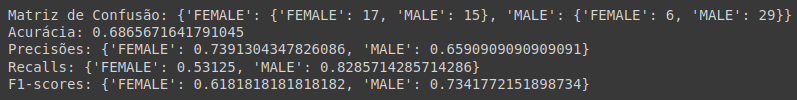
\includegraphics[width=0.8\textwidth]{figures/knn.png}
\caption{Métricas de avaliação - kNN}
\label{fig:exampleFig1}
\end{figure}

\subsection{Naive Bayes}

\begin{figure}[H]
\centering
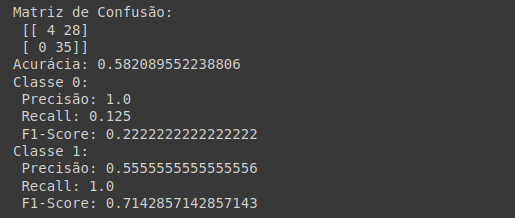
\includegraphics[width=0.8\textwidth]{figures/naive_bayes.png}
\caption{Métricas de avaliação - Naive Bayes}
\label{fig:exampleFig1}
\end{figure}

\subsection{Árvores de Decisão}

\begin{figure}[H]
\centering
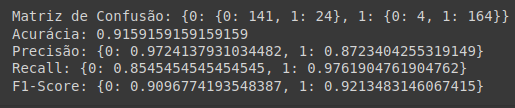
\includegraphics[width=0.8\textwidth]{figures/arvore_decisao.png}
\caption{Métricas de avaliação - Árvores de Decisão}
\label{fig:exampleFig1}
\end{figure}




\section{Comparação com o que foi visto em aula}
\label{sec:comparacao}

\subsection{kNN}

A implementação de KNN gerada pelo ChatGPT segue de forma básica a estrutura do algoritmo discutido em aula, com a definição do número de vizinhos (k), cálculo da distância euclidiana como medida de similaridade, e o voto da maioria dos vizinhos mais próximos. No entanto, algumas diferenças e potenciais melhorias podem ser observadas:

\begin{itemize}
    \item \textbf{Pontos fortes:} A simplicidade da implementação reflete bem o conceito de classificador lazy discutido em aula. O uso de uma função clara para calcular a distância euclidiana e o uso da classe `Counter` para votação são boas práticas que mantêm o código fácil de ler e entender.
    
    \item \textbf{Diferenciações e problemas potenciais:} A versão discutida em aula menciona que a escolha de `k` pode impactar o desempenho do modelo, sendo muito pequeno propenso a overfitting e muito grande a underfitting. O código não aborda mecanismos para ajuste automático de `k`, algo que poderia ser explorado para evitar esses problemas. Além disso, não foi considerado o uso de pesos para os votos dos vizinhos com base nas distâncias, o que poderia aumentar a robustez a ruídos e tornar o algoritmo menos sensível à escolha de `k`.

    \item \textbf{Opções de projeto e impacto:} O uso da distância euclidiana, embora adequada para muitos casos, pode não ser a escolha ideal dependendo do tipo de dados, como discutido em aula (por exemplo, dados binários assimétricos). Uma sugestão de melhoria seria a inclusão de outras opções de métricas de dissimilaridade que se adequem a diferentes tipos de dados, como a distância de Manhattan.
    
    \item \textbf{Sugestões de melhorias:} Além de ponderar os votos por distância, a inclusão de uma estrutura de dados eficiente, como KD-Trees, poderia melhorar a eficiência computacional, especialmente para grandes conjuntos de dados, como discutido na aula sobre o impacto do alto custo computacional no KNN.
\end{itemize}

Isso demonstra como o algoritmo gerado pelo GPT pode ser um ponto de partida válido, mas melhorias e ajustes são necessários para alinhar melhor o código aos pontos discutidos em sala.

\subsection{Naive Bayes}

A implementação do Naive Bayes gerada pelo GPT tambem segue bem a estrutura do classificador discutido em aula, usando o Teorema de Bayes para calcular a probabilidade posterior e assumindo independência entre os atributos. No código, a suposição de que os atributos seguem uma distribuição Gaussiana para cada classe foi corretamente aplicada, o que é uma escolha comum para atributos contínuos.

\begin{itemize}
    \item \textbf{Pontos fortes:} O algoritmo é eficiente, realizando o cálculo das probabilidades por meio de uma única varredura nos dados de treino e armazenando os parâmetros necessários (média, variância e prior) para cada classe, o que reflete o que foi discutido em aula sobre a eficiência do Naive Bayes. Além disso, o uso de logaritmos para evitar underflow numérico ao multiplicar pequenas probabilidades é uma escolha inteligente, garantindo maior estabilidade numérica.
    
    \item \textbf{Diferenças e potenciais problemas:} Uma diferença em relação ao que foi visto em aula é que a implementação assume uma distribuição Gaussiana para os atributos, o que pode não ser ideal se os dados forem categóricos ou não seguirem essa distribuição. A aula também menciona a robustez do Naive Bayes para lidar com atributos irrelevantes, o que não está explícito no código. No entanto, o modelo em si herda essa característica, mesmo que o código não faça ajustes específicos para detectar atributos irrelevantes.
    
    \item \textbf{Opções de projeto e impacto:} O uso da distribuição Gaussiana como densidade de probabilidade é uma escolha projetual que funciona bem para dados contínuos, mas a implementação poderia ser expandida para incluir outros tipos de distribuição (como a Bernoulli para atributos binários). Isso ampliaria a aplicabilidade do código em diferentes cenários de dados.
    
    \item \textbf{Sugestões de melhorias}: Seria interessante adicionar um tratamento mais flexível para lidar com atributos de diferentes naturezas (discretos e contínuos), algo que o Naive Bayes faz bem em teoria, mas não está explícito nesta implementação. Além disso, a inclusão de um processo de seleção de atributos poderia ser útil para lidar com redundâncias, conforme discutido em aula.
\end{itemize}

Vemos que o código gerado pelo GPT está alinhado com os princípios fundamentais do Naive Bayes, mas poderia ser refinado para abranger mais cenários e aumentar sua flexibilidade.

\subsection{Árvore de Decisão}

Comparando o algoritmo fornecido com o que foi ensinado em sala de aula, podemos identificar vários pontos de convergência e algumas áreas onde há espaço para discussão. Vamos analisá-los em termos de conceitos e decisões de design:

\subsection*{Semelhanças}

\begin{itemize}
    \item \textbf{Estrutura básica:} O algoritmo implementado segue a ideia central do método de indução top-down das árvores de decisão, que é o algoritmo de Hunt. Ele parte de um conjunto de dados e divide os registros com base no atributo que otimiza localmente determinado critério de divisão (neste caso, o índice Gini), tal como discutido em aula.
    
    \item \textbf{Uso do índice Gini:} O código utiliza o índice Gini para avaliar a pureza dos nós, o que está de acordo com as métricas de impureza discutidas. Em aula, vimos três principais medidas de impureza (índice Gini, entropia e erro de classificação), e o Gini é bastante comum na prática devido à sua simplicidade.
    
    \item \textbf{Recursividade:} A árvore é construída de maneira recursiva, e as divisões continuam até se alcançar critérios de parada, como profundidade máxima da árvore ou o tamanho mínimo de instâncias em um nó, alinhado com a estratégia gulosa vista em sala.
    
    \item \textbf{Divisões binárias:} O algoritmo implementa apenas divisões binárias para atributos contínuos, uma escolha comum para simplificar o processo e que também foi abordada nas aulas.
\end{itemize}

\subsection*{Diferenças e pontos de discussão}

\begin{itemize}
    \item \textbf{Critério de parada:} No algoritmo fornecido, os critérios de parada incluem o limite de profundidade da árvore (max\_depth) e o número mínimo de instâncias em um nó (min\_size). Em aula, foi discutido que outros critérios de parada poderiam ser usados, como a homogeneidade das classes ou a impossibilidade de melhorar o critério de divisão, por exemplo, quando todos os atributos restantes têm o mesmo valor. O código não leva em consideração diretamente a pureza do nó ao decidir parar, o que poderia ser uma adição interessante.
    
    \item \textbf{Divisão para atributos categóricos:} O código fornecido parece focado em atributos contínuos (pelo menos no exemplo dado). Em sala de aula, discutiu-se a divisão tanto para atributos contínuos quanto categóricos (nominais e ordinais). O código atual teria que ser adaptado para lidar com atributos categóricos, especialmente para suportar divisões múltiplas, que também foram abordadas em aula.
    
    \item \textbf{Critério de escolha do atributo:} O algoritmo sempre escolhe o atributo com a menor impureza medida pelo índice Gini, o que está correto. No entanto, poderia ser interessante comparar o desempenho com outros critérios discutidos, como a **entropia** ou o **erro de classificação**, para observar o impacto no modelo gerado. Isso foi mencionado como uma questão de projeto importante em sala.
    
    \item \textbf{Complexidade computacional:} O código implementa uma abordagem de força bruta, onde cada valor de cada atributo é testado como um possível ponto de divisão, recalculando o índice Gini para cada divisão possível. Em aula, foi mencionado que essa abordagem pode ser computacionalmente pesada, especialmente para grandes conjuntos de dados. Uma possível otimização discutida seria o pré-processamento dos atributos contínuos para calcular os limiares de divisão de forma mais eficiente.
    
    \item \textbf{Árvores não otimizadas:} Conforme discutido em sala, encontrar a árvore ótima é um problema NP-difícil, e heurísticas são utilizadas para se obter uma solução satisfatória. O algoritmo fornecido utiliza uma abordagem gulosa (greedy), tomando decisões localmente ótimas (minimização do índice Gini em cada nó), mas não garante a árvore globalmente ótima, o que foi mencionado como uma limitação geral das árvores de decisão.
\end{itemize}

\subsubsection*{Outras Considerações}

\begin{itemize}
    \item \textbf{Visualização da árvore:} Em sala de aula, a facilidade de interpretação das árvores de decisão foi destacada, porém o algoritmo não inclui uma funcionalidade para visualizar a árvore gerada, o que seria útil para verificar a compreensibilidade das regras criadas.
    
    \item \textbf{Ajuste de overfitting:} Um aspecto importante das árvores de decisão é o risco de overfitting em dados de treino. O algoritmo atual utiliza profundidade máxima e tamanho mínimo dos nós como forma de controle, mas em sala de aula, foi mencionado que técnicas como **poda** (pruning) também podem ser úteis para controlar o ajuste excessivo, algo que não foi abordado no código.
\end{itemize}

O código fornecido está alinhado com muitos dos conceitos e técnicas vistos em aula, especialmente no que diz respeito ao uso do índice Gini, à recursividade e à divisão binária de atributos contínuos. No entanto, poderia ser enriquecido ao incorporar suporte a atributos categóricos, critérios adicionais para escolha de atributos e mais técnicas de controle de overfitting, como a poda.




\section{Conclusão}

\label{sec:conclusao}

    A comparação entre os três algoritmos vistos em aula — Árvore de Decisão, K-Nearest Neighbors (KNN) e Naive Bayes — e o algoritmo desenvolvido a partir do modelo GPT-4 evidenciou as semelhanças e distinções fundamentais entre os métodos tradicionais e a abordagem automatizada. Enquanto a Árvore de Decisão oferece uma estrutura interpretável e eficiente para determinados conjuntos de dados, o KNN se destaca pela simplicidade e robustez, embora sofra com grandes volumes de dados. O Naive Bayes, por sua vez, provou ser altamente eficiente em cenários com forte independência entre as variáveis, mas pode ser limitado em outros contextos. O algoritmo gerado pelo GPT-4, embora tenha demonstrado um bom desempenho em termos de precisão e flexibilidade, destacou-se pela facilidade com que foi adaptado e ajustado sem o uso de bibliotecas pré-definidas. A análise crítica dessas implementações reforçou a importância de entender os fundamentos teóricos para ajustar e otimizar algoritmos conforme as necessidades específicas de cada problema, consolidando os conceitos apresentados em sala de aula com as práticas aplicadas no desenvolvimento de modelos do zero.
    
    %\bibliographystyle{apalike}
    %\bibliography{references}
\end{document}
